\notechapter{N-20220323}{Complex Differentiability and the Rigidity of Holomorphic Functions}

\section{Why complex analysis feels different}

Real analysis contains many pathological examples:
\begin{enumerate}[(i)]
  \item the Cantor function is continuous, has derivative zero almost everywhere, yet is not constant;
  \item the Weierstrass function is continuous everywhere and differentiable nowhere;
  \item a function may have many derivatives but fail at the next derivative;
  \item a smooth real function may have a Taylor series that does not recover the function.
\end{enumerate}

For example,
\[
  f(x)=
  \begin{cases}
    e^{-1/x},&x>0,\\
    0,&x\le0
  \end{cases}
\]
is smooth, but its Taylor series at \(0\) is identically zero and therefore does not equal \(f\) for \(x>0\).

Complex analysis is much more rigid.  Holomorphic functions behave as if a tiny amount of local data can determine a large amount of global behavior.

\section{Complex derivative}

\begin{definition}
Let \(U\subseteq\mathbb C\) and \(f:U\to\mathbb C\).  The derivative of \(f\) at \(z_0\in U\) is
\[
  f'(z_0)=\lim_{h\to0}\frac{f(z_0+h)-f(z_0)}{h},
\]
provided the limit exists.
\end{definition}

The key difference from real differentiability is that \(h\) approaches \(0\) through the complex plane, not merely from the left and right along a line.  The quotient must have the same limit from every direction.

\begin{figure}[H]
  \centering
  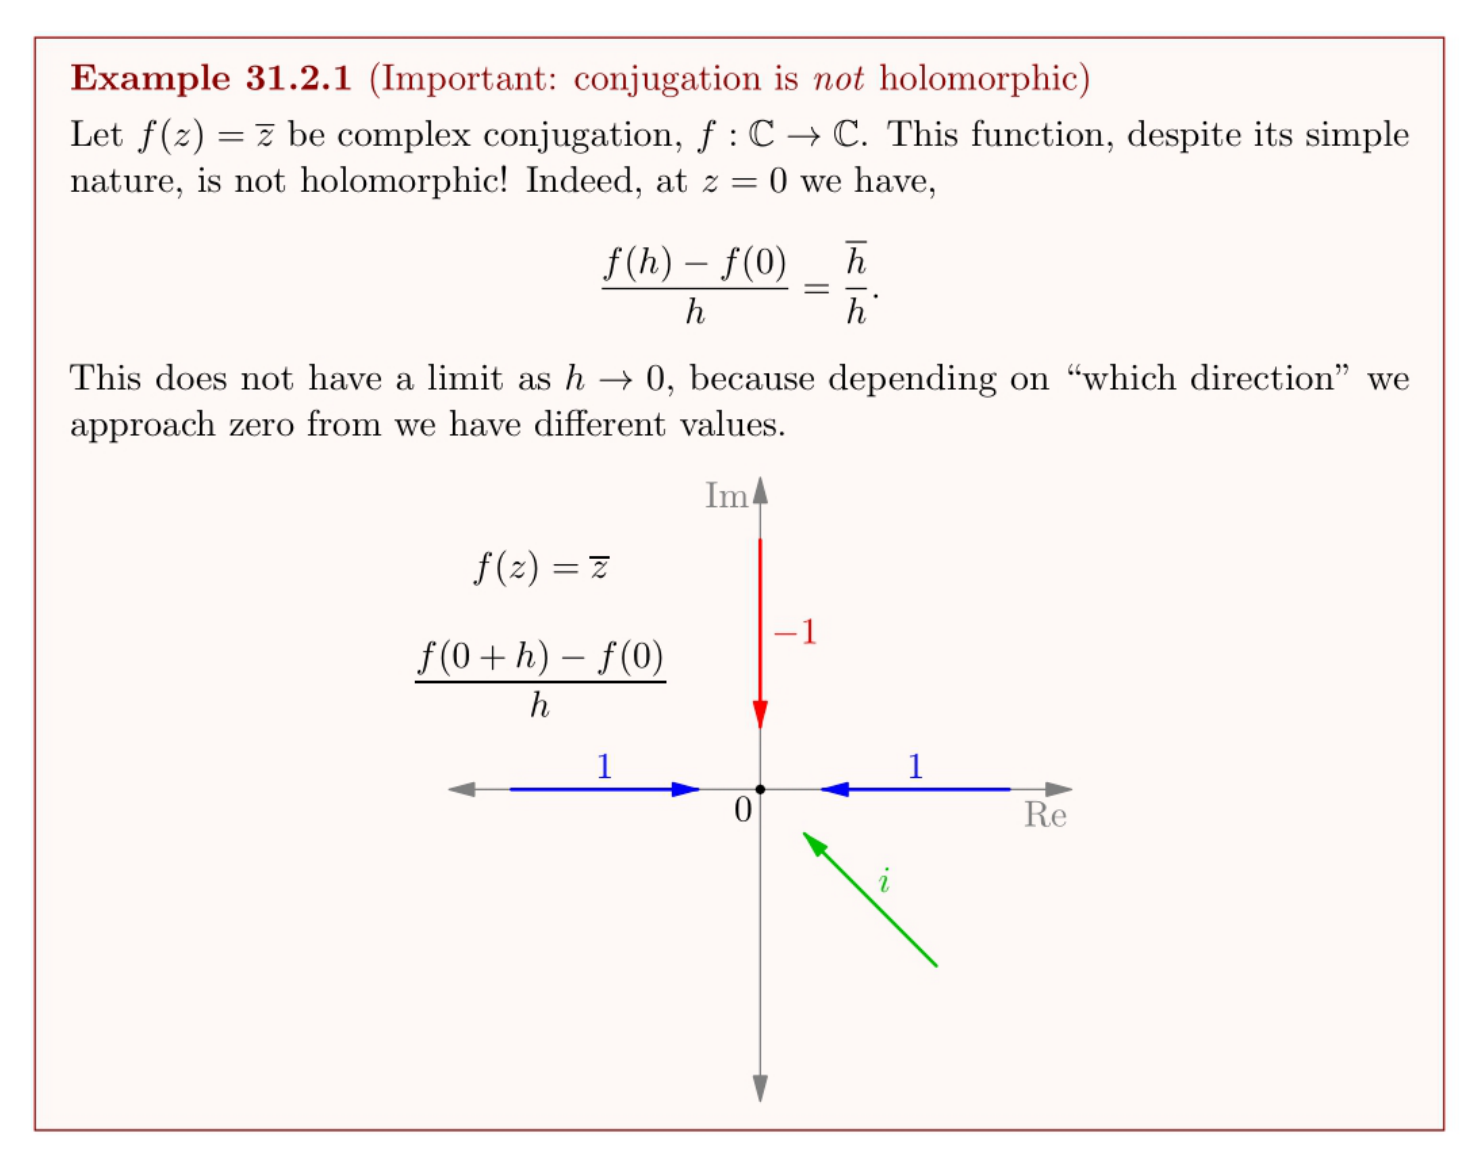
\includegraphics[width=0.80\textwidth]{figures/N-20220323/fig-01.png}
  \caption{In complex differentiability, the increment approaches from all directions in the plane.}
\end{figure}

\begin{definition}
A function \(f:U\to\mathbb C\) is holomorphic if it is complex differentiable at every point of \(U\).  If \(U=\mathbb C\), then \(f\) is called entire.
\end{definition}

\section{Basic examples}

\begin{example}
Every polynomial
\[
  a_nz^n+a_{n-1}z^{n-1}+\cdots+a_0
\]
is holomorphic.
\end{example}

\begin{example}
The complex exponential is holomorphic.  In real and imaginary parts,
\[
  e^{x+iy}=e^x(\cos y+i\sin y).
\]
\end{example}

\begin{example}
The trigonometric functions extend holomorphically to the complex plane by
\[
  \cos z=\frac{e^{iz}+e^{-iz}}{2},
  \qquad
  \sin z=\frac{e^{iz}-e^{-iz}}{2i}.
\]
\end{example}

\section{Closure properties}

Holomorphic functions are closed under the usual operations:
\begin{enumerate}[(i)]
  \item sums of holomorphic functions are holomorphic;
  \item products of holomorphic functions are holomorphic;
  \item quotients are holomorphic wherever the denominator is nonzero;
  \item compositions of holomorphic functions are holomorphic.
\end{enumerate}

\begin{remark}
This resembles real calculus formally, but the consequences are stronger.  Complex differentiability is a much more restrictive condition than real differentiability.
\end{remark}

\section{The main intuition}

The main point of this note is that complex differentiability is not merely ordinary differentiability with complex numbers inserted.  Requiring the difference quotient to approach the same value from every complex direction forces strong compatibility conditions, later expressed by the Cauchy--Riemann equations.

\begin{remark}
The next step should be to derive the Cauchy--Riemann equations and then explain why holomorphic functions are analytic.  This will make precise the slogan that complex functions are rigid.
\end{remark}


\section{Complex differentiability is stronger than real differentiability}

A complex function \(f(z)=u(x,y)+iv(x,y)\) is real differentiable as a map \(\mathbb R^2\to\mathbb R^2\) if it has a real linear approximation.  It is complex differentiable if that linear approximation is multiplication by a complex number.  This extra requirement forces the Cauchy--Riemann equations:
\[
  u_x=v_y,\qquad u_y=-v_x.
\]
Thus holomorphic functions are far more rigid than arbitrary differentiable two-variable functions.

\section{Local power series intuition}

Once a function is holomorphic on a disk, it is represented by a power series there.  This is the source of many surprising consequences: holomorphic functions are infinitely differentiable, zeros are isolated unless the function is identically zero, and values on small sets can determine the function globally.
